\chapter{Estado de los recursos}
\label{chap:estadoInfraestructuraSistema}
\lettrine{C}{on} el fin de contextualizar los recursos que se utilizarán en este trabajo, en este capítulo se expone la situación actual de toda la infraestructura en lo relacionado al software que está en funcionamiento, a los recursos físicos de los que se compone, y al estado actual de las herramientas que rodean a dichos recursos.

\section{Infraestructura}
La infraestructura física de este servicio de Cloud Computing, se encuentra localizada en el edificio del CITIC de la UDC, dentro de un rack alojado en su Centro de Proceso de Datos (CPD) \cite{citicUDC}. Está formado por 5 nodos \textit{Lenovo NeXtScale nx360 M5} y 3 nodos \textit{Dell EMC PowerEdge R740}. Ambos componentes dan flexibilidad en cuanto a la escalabilidad y ofrecen gran rendimiento de cómputo.\\

Especificaciones principales de los nodos:
\begin{itemize}
    \item Lenovo NeXtScale nx360 M5: 
        \begin{itemize}
            \item CPU: Dos Intel Xeon E5-2650
            \item Memoria: 128 GB
            \item Tarjeta  gráfica: Tesla M60
        \end{itemize}
            Más información: \url{https://lenovopress.com/tips1195-nextscale-nx360-m5-e5-2600-v3}
    \item Dell EMC PowerEdge R740:
        \begin{itemize}
            \item CPU: Dos Xeon Gold 6146
            \item Memoria: 384 GB
            \item Tarjeta gráfica: Tesla P40
        \end{itemize}
    Más información: \url{https://www.dell.com/es-es/work/shop/servidores-almacenamiento-y-redes/smart-value-poweredge-r740-server-standard/spd/poweredge-r740/per7400m}
\end{itemize}
El almacenamiento está colocado físicamente en la misma ubicación que los hosts pero en su abstracción lógica este es independiente y está separado de cada nodo. Está conformado por 13 discos duros SSD de 3.84 TB de capacidad, obteniendo así una capacidad total de casi 50 TB, pero que utilizan el sistema de almacenamiento RAID 5[Pal. \ref{itm:raid5}] lo cual permite conseguir mayor  integridad de los datos, tolerancia a fallos y ancho de banda, reduciendo la cantidad de almacenamiento utilizable a 34 TB. Estos discos forman un \textit{pool} de almacenamiento que se divide en cinco LUNs (\textit{Logical Storage Unit})[Pal. \ref{itm:lun}] de 2 TB cada una, representadas en el sistema de virtualización como cinco \textit{datastores} diferentes que utilizan el sistema de archivos VMFS el cual optimiza el almacenamiento de máquinas virtuales.\\
Los discos duros físicos están colocados en una misma cabina y son accesibles por todos los nodos a través de dos switches para aportar redundancia. Para ello, las cabinas incorporan dos controladores SFP+[Pal. \ref{itm:sfp}] que se conectan a cada switch mediante dos puertos que aportan conectividad 10 Gb y, además, incorporan otros dos puertos con conectividad 1 Gb para la gestión de los discos. Estas conexiones utilizan los protocolos de red Ethernet y iSCSI, formando así, junto con el resto de componentes descritos, la estructura de una SAN [\ref{fig:esquemaentornoreal}].\\

La gestión del almacenamiento se realiza en la capa física, el nivel más bajo por lo que la configuración de cada LUN que utilizan las máquinas virtuales desplegadas se tiene que hacer antes de conocer los requisitos necesarios de lo que se vaya a desplegar en la capa software. Esto provoca que si se quiere desplegar una máquina virtual con más capacidad de almacenamiento o con una estructura RAID diferente haya que crear una nueva LUN que se adapte a los requisitos.
Esta gestión hace que el uso de recursos de almacenamiento no sea el óptimo ya que no permite ajustar de forma precisa y rápida cada configuración a los requisitos necesarios generando así mayor coste.

\iffalse
Los nodos acceden a los discos de almacenamiento a través de dos switches que al mismo tiempo dan conectividad entre los nodos formando una SAN. Los 10TB de capacidad están repartidos entre cinco DataStores, de 2TB cada uno. Una máquina virtual está alojada en un DataStore concreto pero puede tener ficheros alojados en varios almacenes de datos diferentes.
Las conexiones entre dispositivos son Ethernet 10 Gigabit combinado con el protocolo de transporte ISCSI
\fi

\section{Software}
\label{subsec:softwareinstalado}
Actualmente el servicio está basado en el software de la empresa VMware, uno de los principales proveedores de software de virtualización, siendo \textbf{VMware vSphere} el software desplegado sobre la infraestructura. Este producto de VMware es el encargado de virtualizar parte de la infraestructura física y de proporcionar las herramientas necesarias para gestionarla. Sus \underline{principales componentes} son los siguientes:
\begin{itemize}
    
    \item \textbf{ESXi}: Hipervisor propio de VMware, de tipo 1 o \textit{bare metal}[Pal. \ref{itm:baremetal}]. No requiere de sistema operativo para funcionar ya que funciona directamente sobre el hardware físico\cite{Esxi}. Este hipervisor está instalado en cada uno de los cinco nodos que forman la infraestructura.
    
    \item \textbf{VMware vCenter Server}: servicio que actúa como un administrador central para todas las máquinas virtuales y hosts. Normalmente, los servicios descritos en este apartado están disponibles para una instancia de vCenter Server agrupados en un \textit{Platform Services Controller} (PSC) [Pal. \ref{itm:psc}]
    
    \item \textbf{vCenter Single Sign-On}: es un servicio de autenticación. Permite que los usuarios solo se tengan que autenticar una vez cuando acceden al entorno de la infraestructura a través de vSphere Client, en lugar de tener que autenticarse varias veces en cada componente. Cuando el usuario se autentica por primera vez, este recibe un token que le permitirá autenticarse en el resto de componentes sin volver a introducir sus credenciales. También se encarga de la administración perfiles de usuarios y de los dominios de autenticación (esto permite usar directorios de usuarios externos).\label{itm:singlesingonEX}
    
    \iffalse
    \item \textbf{vSphere License Server}: permite gestionar e inventariar licencias para aquellos sistemas conectados a un \emph{Platform Services Controller}.
    
    \item \textbf{VMware Certificate Authority}: provee con un certificado a cada nodo. está firmado por esta misma autoridad (VMCA).
    \fi
    \iffalse
    \item \textbf{PostgreSQL}: distribución de la base de datos PostgreSQL para vSphere.
    \fi
    \item \textbf{vSphere Web Client} y \textbf{vSphere Client}: interfaz que permite conectarse a una instancia de vCenter Server para gestionar la infraestructura.
    
    
    \iffalse
    \item \textbf{vSphere ESXi Dump Collector}: permite configurar un host ESXi para que guarde su memoria en un servidor externo en lugar de en un disco cuando hay algún fallo crítico.
    \item \textbf{vSphere Syslog Collector}: habilita logs de red. 
    \fi
    \item \textbf{vSphere Auto Deploy}: herramienta que permite desplegar gran cantidad de nodos físicos de forma automátizada.
    
    \item \textbf{vSphere Update Manager Extension}: centraliza y gestiona las actualizaciones de todos los objetos de vSphere. Con Update Manager se pueden aplicar actualizaciones a los hosts ESXi, instalar y actualizar software de terceros en los hosts, y actualizar el hardware de una máquina virtual.
   
    \item \textbf{vSphere Web Client}: interfaz web que permite acceder a vCenter Server de forma remota.
    
    \item \textbf{vMotion}: permite la migración de máquinas virtuales de un host a otro de forma transparente y sin detener su ejecución. Este servicio también es usado por vSphere Hight Availability para migrar las máquinas virtuales cuando un host no está disponible.
    
    \item \textbf{Storage vMotion}: permite migrar los discos y configuración de una máquina virtual de un \textit{datastore} a otro sin interrumpir el servicio.
    
    \item \textbf{vSphere High Availability (HA)}: provee alta disponibilidad para las máquinas virtuales. En caso de que una máquina virtual deje de estar activa este servicio la reinicia en otro host dentro del mismo cluster automáticamente. Proporciona escalabilidad gracias a su modelo Maestro - Esclavo, fiabilidad gracias a que no tiene dependencias con otros servicios y a que se puede comunicar con las máquinas a través de varios caminos, y usabilidad gracias a que tiene una interfaz sencilla.
    
    \item \textbf{vSphere Distributed Resource Scheduler (DRS)} y \textbf{vSphere Distributed Power Management (DPM)}: DRS genera recomendaciones sobre donde se debería desplegar una máquina virtual cuando se está creando, mueve las máquinas virtuales a través de los hosts de un cluster para maximizar el rendimiento o durante tareas de mantenimiento en un host. DPM se encarga de gestionar el consumo de energía de cada host según el rendimiento necesario.
    \item \textbf{Storage DRS}: balancea la carga de almacenamiento y las operaciones I/O entre los diferentes datastores disponibles.
    
    \item \textbf{vSphere Fault Tolerance}: crea una copia de todos los archivos y discos de cada máquina virtual sincronizados con los originales. Esto junto con vSphere HA y vSphere DRS, proporciona recuperación ante fallos y  disponibilidad continua de las máquinas virtuales, realizado de forma automática en caso de fallos, sin perdida de datos y sin pérdida de conexiones de la máquina virtual. Este servicio está orientado a proteger aquellas tareas que requieren un alto rendimiento o que son críticas. habilitadas creando una copia de cada una  para usarla en caso de que la primera falle.
    
    \item \textbf{Distributed Switch (vDS)}: habilita swithces virtuales que se encargan de gestionar el tráfico de los hosts ESXi.
    
    \item \textbf{Virtual Machine File System (VMFS)}: sistema de archivos de alto rendimiento nativo de VMware vSphere. Se utiliza para implementar los almacenes de datos de la infraestructura y está optimizado para el almacenamiento de máquinas virtuales.
\end{itemize}

\begin{figure}[hp]
  \centering
  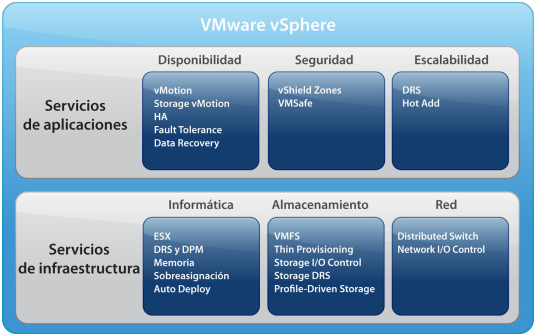
\includegraphics[width=0.75\textwidth]{imaxes/cap2recursos/contentVSphere}
  \caption{Elementos de la plataforma VMWare vSphere\cite{fotovSphere}}
  \label{fig:componentesVSphere}
\end{figure}
\begin{figure}[hp]
  \centering
  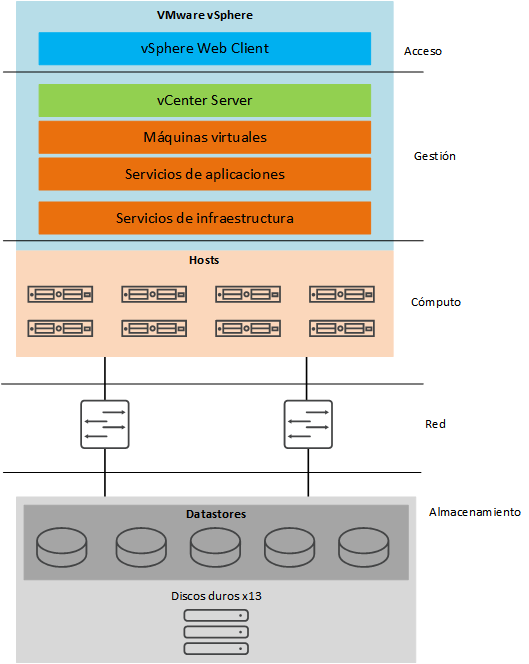
\includegraphics[width=1\textwidth]{imaxes/cap2recursos/recursosReal.png}
  \caption{Esquema de los recuros software y hardware del entorno}
  \label{fig:esquemaentornoreal}
\end{figure}

\FloatBarrier
\subsection{Estado de la tecnología}

En los últimos tiempos los servicios de \textit{Infrastructure as a Service} (IaaS) se han extendido de forma considerable con la aparición de software que permite la gestión de un sistema de Cloud Computing, como pueden ser VMware Cloud Foundation (2011), OpenStack (2010), o Apache CloudStack (2012). Estas herramientas construyen una infraestructura virtual sobre un entorno físico estandarizado que les permite administrar y automatizar la escalabilidad, el sistema de almacenamiento, la disponibilidad del servicio, la red, y la seguridad del servicio, con lo que se consigue reducir el coste y el tiempo de gestión y configuración, mejorando la eficiencia de infraestructura física.

A la hora de alcanzar los objetivos descritos en este proyecto se nos plantea la duda de que solución software desplegar ya que actualmente existen tres principales alternativas en el mercado, VMware Cloud Foundation, OpenStack y Apache CloudStack. Cada una de ellas ofrece diferentes características con diferentes requisitos que se pueden adaptar mejor o peor al entorno de despliegue, pero después de comprobar esos aspectos tenemos claro que la \underline{solución elegida es VMware Cloud Foundation}.

\subsubsection{VMware Cloud Foundation}
Esta solución virtualiza todas las capas de la infraestructura[Fig. \ref{fig:infraCloudFound}] (red, computación y almacenamiento) combinando cuatro componentes principales, vSphere para gestionar el cómputo, vSAN para la gestión del almacenamiento, NSX para la gestión de la red, y vRealize para gestionar todas las operaciones que tienen lugar en el servicio, integrando todos los componentes para que la gestión de la infraestructura sea lo más simple posible. Este cojunto de herramientas convierten el CPD en un \textit{Software Defined Datacenter} (SDDC), un entorno donde todas las partes físicas de la infraestructura pasan a estar controladas a través de software haciendo más flexible, independiente y menos costosa la configuración de estos componentes[Fig. \ref{fig:sddcoverview}]. Las \underline{principales características} de VMware Cloud Foundation son:
\begin{itemize}
    \item \textbf{Servicios software con integración nativa}: ofrece un conjunto de servicios software para el almacenamiento, red, seguridad y gestión de la cloud. Estos servicios se integran de forma nativa con la infraestructura minimizando las tareas de configuración y administración.
    \item \textbf{Escalabilidad y elasticidad de los recursos}: la capacidad de la infraestructura se puede modificar de forma sencilla gracias a la automatización del ciclo de vida de todos los elementos. 
    \item \textbf{Supervisión de los recursos}: ofrece supervisión de los recursos con reconocimiento de aplicaciones y solución de problemas, permitiendo conocer todos los eventos que tienen lugar en la infraestructura.
    \item \textbf{Aprovisionamiento de automatizado}: todos los componentes necesarios para formar un SDDC son desplegados automáticamente por VMware Cloud Foundation, incluyendo los recursos informáticos, los componentes de almacenamiento, los de red y los de administración.
    \item \textbf{Ciclo de vida automatizado}: automatiza las operaciones previas, iniciales y posterios de una plataforma de software para ofrecer una gestión más sencilla. Esto incluye su implementación, el aprovisionamiento de clústeres aislados bajo demanda y la instalación de actualizaciones y parches.
   
   \iffalse 
    \item \textbf{Experiencia de usuario simple}: gracias a la gran cantidad de procesos automatizados.
    \item \textbf{Escalabilidad modular}: el sistema y la infraestructura se puede escalar de forma sencilla.
    \item \textbf{Cloud híbrida}: da la posibilidad de conectar una Cloud pública con una Cloud privada y así tratar ambas como una única Cloud.
    \fi
\end{itemize}

\begin{figure}[h!]
  \centering
  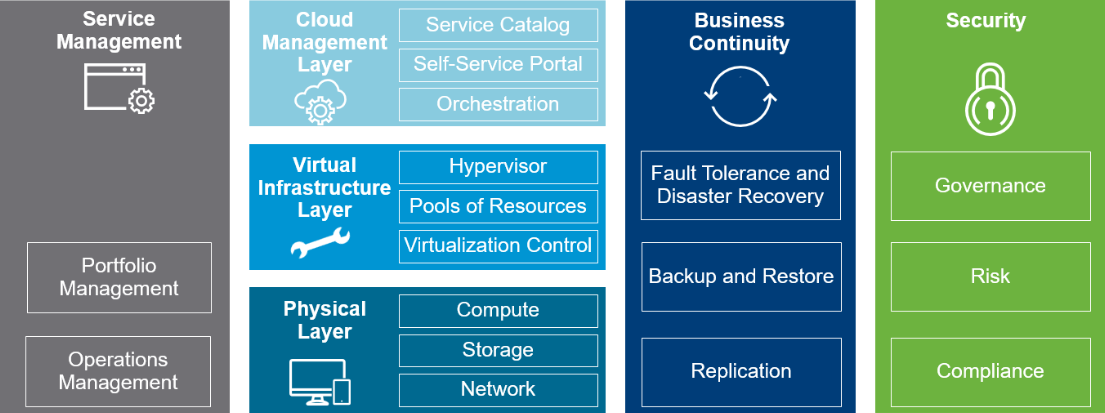
\includegraphics[width=1\textwidth]{imaxes/cap2recursos/SDDCoverview.png}
  \caption{Partes virtualizadas en un SDDC.}
  \label{fig:sddcoverview}
\end{figure}
\\
\begin{figure}[h!]
  \centering
  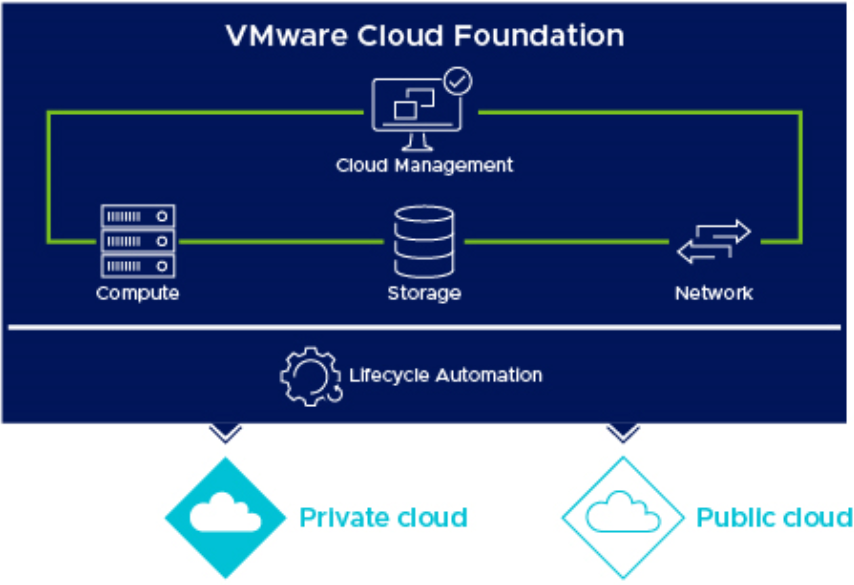
\includegraphics[width=1\textwidth]{imaxes/cap2recursos/overviewCF.png}
  \caption{Cloud Foundation virtualiza toda la infraestructura.}
  \label{fig:infraCloudFound}
\end{figure}

VMware Cloud Foundation permite reducir el tiempo de mantenimiento ya que todo está controlado por el software que integra todos los componentes, automatizando gran parte de las operaciones y el ciclo de vida de todos los elementos desde su creación, como puede ser el control de versiones de cada elemento, los perfiles de usuario y las máquinas virtuales creadas, además de proporcionar una plataforma de acceso para que cada usuario pueda gestionar sus recursos.

*****************************************************\\
También permite separar las cargas de trabajo mediante Dominios según el tipo de trabajo que se va a realizar, pudiendo acceder a cada uno de ellos de forma separada.\\
*****************************************************\\

Para poder usar este software es necesaria la adquisición de licencias, estas se organizan por componente y por número de hosts sobre los que se va a instalar el producto, haciendo que el coste sea elevado, pero, a pesar de eso, se ha elegido este paquete principalmente por su integración nativa con los componentes ya instalados y porque su mantenimiento es más sencillo. \\
Si bien VMware ofrece plugins para conectar sus componentes con otras soluciones, como es el caso de OpenStack \cite{opestackintegrated}, estos no ofrecen el rendimiento que da la integración nativa, además, en caso de recibir actualizaciones, habría que actualizar cada componente de forma individual aumentando el riesgo de incompatibilidades con el resto de elementos del sistema, mientras que Cloud Foundation gestiona todo el ciclo de vida de cada actualización para cada componente, permitiendo comprobar si existe alguna incompatibilidad con el resto de versiones antes de aplicar una actualización. En definitiva, VmWare Cloud Foundation simplifica el proceso de instalación, configuración, gestión, y mantenimiento, tanto para los usuarios como para el administrador del sistema.

\subsubsection{Componentes de VMware Cloud Foundation \cite{componentesCloudFound}}
\label{subsubsect:cfcomponents}
\begin{itemize}
    \item \textbf{SDDC Manager}: gestiona el ciclo de vida de todos los componentes del sistema, incluyendo el proceso inicial de despliegue de Cloud Foundation, su configuración y aprovisionamiento, y las actualizaciones. Monitoriza los recursos físicos y lógicos de la infraestructura, facilita su configuración y permite añadir nuevos recursos cuando sea necesario. \iffalse Todo esto lo realiza mediante flujos de trabajo que facilitan la detección de orígenes de errores.\fi
    \item \textbf{vSphere}: ya está incluído en el servicio actual [\ref{subsec:softwareinstalado}].
    \item \textbf{VMware vSAN}: componente clave que virtualiza el almacenamiento. Como ya se ha explicado, el almacenamiento del servicio actual está configurado con LUNs que se deben gestionar individualmente en una capa distinta a los componentes software, provocando que su configuración sea más compleja y costosa. El objetivo de VMware vSAN es gestionar de forma automatizada y desde un único lugar el sistema de almacenamiento de la infraestructura, tratando toda la capacidad y recursos de almacenamiento como un único elemento, eliminando así la necesidad de tener que crear LUNs aisladas, consiguiendo abstraer la configuración de almacenamiento de la capa física en la capa de software y permitiendo establecer políticas de almacenamiento desde cada máquina virtual para adecuarlo a las necesidades de cada una sin tener que editar la configuración real del entorno físico. Así el rendimiento de los recursos de almacenamiento es más eficiente, flexible y su configuración se integra dentro del mismo servicio junto con la gestión del resto de componentes. \\
    En vSAN, en lugar de tratar el almacenamiento de forma independiente este pasa a estar ligado a cada host, es decir, cada uno de los nodos tiene asignados hasta cinco grupos de discos. Estos grupos de discos pueden ser híbridos, donde se combinan discos duros SSD y HDD, o All-Flash, donde todos los discos utilizan tecnología \textit{Solid-State Drive} (SSD). Dentro de cada grupo hay \underline{dos tipos de discos} con distintas funciones, el disco de caché y el disco de capacidad\cite{operacionesVSAN}:
        \begin{itemize}
            \item \textbf{Caché}: Hay uno en cada grupo. Realiza la función de memoria caché y se encarga de escribir los datos persistentes en los discos de capacidad.
            \item \textbf{Capacidad}: Puede haber hasta siete discos en cada grupo. Almacena los datos persistentes del entorno.
        \end{itemize}
    En cada grupo de discos la gestión de la \underline{lectura y escritura} de datos se hace de la siguiente forma:
        \begin{itemize}
            \item \textbf{Lectura}: En el caso de la solución híbrida, si el dato que se busca no está en el disco de caché entonces se busca en los discos de capacidad y después se incorpora al disco de caché. Con la solución all-flash, los datos se leen siempre directamente de los discos de capacidad sin que estos sean escritos en el disco de caché dejando a este completamente libre para las operaciones de escritura. Gracias a esto, la estructura all-flash ofrece mayor rendimiento respecto a la híbrida.
            \item \textbf{Escritura}: Tanto en la solución híbrida con en la all-flash, el host ESXi primero escribe en el disco de caché, este le responde con una confirmación de escritura y más tarde vSAN se encarga de escribir ese dato en los discos de capacidad cuando el disco de caché está casi completo o cuando el dato lleva un tiempo sin ser utilizado.
        \end{itemize}
        \begin{figure}[h!]
            \centering
            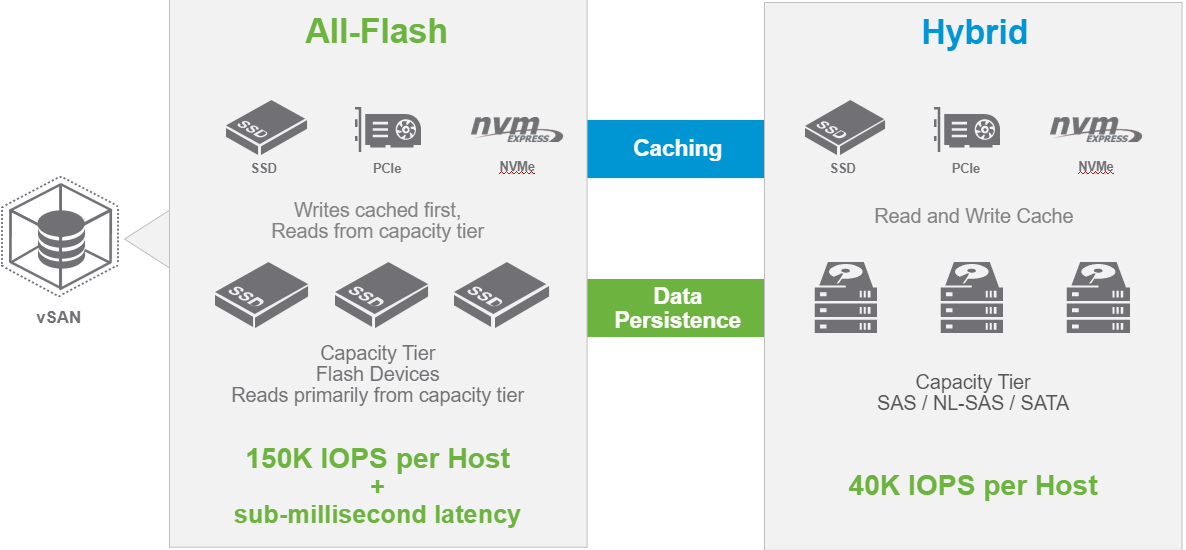
\includegraphics[width=1\textwidth]{imaxes/cap2recursos/rendimientoVSAN.png}
            \caption{Almacenamiento All-Flash vs. Híbrido en vSAN}
            \label{fig:rendimientoVSAN}
        \end{figure}
        \FloatBarrier
    Los hosts acceden al \textit{datastore} de vSAN mediante protocolo IP en una red accesible por todos los nodos. \\ 
    Este componente permite reducir las tareas de gestión del almacenamiento físico ya que ya no es necesario hacer ajustes en la capa física para cumplir unos requisitos en la capa software.
    \item \textbf{VMware NSX}: otro de los componentes clave. Tiene un papel similar a vSAN, pero en este caso se encarga de virtualización de los componentes físicos de la red de la infraestructura, es decir, abstrae los componentes físicos de nuestro entorno en software, dando más libertad a la hora de establecer la topología y componentes físicos de la red. Incluye servicios como firewall, DNS, DHCP, VPN, NAT, enrutamiento, balanceo de carga, o switching, que permiten reducir la cantidad de dispositivos físicos de red.\\
    Principales \underline{componentes internos}\cite{componentesNSX}:
    \begin{itemize}
        \item \textbf{NSX Manager}: permite crear, configurar y administrar el resto de recursos de NSX. Su interfaz está integrada en vSphere.
        \item \textbf{NSX Controller}: contiene las tablas de ARP, MAC, VTEP y de enrutamiento.
        \item \textbf{NSX Virtual Switch}: gestiona los vSphere vSwitch Distibuted desplegados, proporcionando switching a los nodos ESXi.
        \item \textbf{NSX Logical Router Control}: se despliega cuando se crea un Distributed Logical Router. Se encarga de buscar adyacencias para generar tablas de enrutamiento que envía a NSX Manager y a los NSX Cotrollers para que informen a cada Distributed Logical Router en cada nodo ESXi.
        \item \textbf{NSX Edge}: proporciona servicios múltiples servicios como firewall perimetral de capa 2 y 3, SSL, NAT, DHCP, VPN, balanceo de carga y alta disponibilidad.
    \end{itemize}
    \item \textbf{VMware vRealize Log Insight}: realiza la gestión de logs del servicio, dando visibilidad a todas las operaciones del servicio, generando análisis del sistema. Esto permite tener mayor conocimiento de los riesgos, eficiencia y uso de recursos, a parte de facilitar la búsqueda de orígenes de errores.\\
    Para su correcto funcionamiento \underline{requiere desplegar los siguientes componentes}:
    \begin{itemize}
        \item \textbf{Nodo Master}: cuando se despliega con el modo \textit{standalone} este el responsable de todas las actividades, incluyendo las consultas y gestión de logs. También participa en la gestión del ciclo de vida del cluster actualizando, eliminando y añadiendo nodos \textit{Worker}. 
        \item \textbf{Nodo Worker}: se generan para proporcionar alta disponibilidad facilitando la escalabilidad del entorno. En estos nodos se delegan las tareas de consulta y gestión de logs.
        \item \textbf{Load Balancer}: se encarga de centralizar y asegurar la entrada de logs en Log Insight simplificando la configuración para habilitar la alta disponibilidad. También balancea el tráfico de logs entrante entre los nodos existentes.
    \end{itemize}
\end{itemize}

**Decir como se puede implementar un sistema de facturación.*******\\
**Como se puede conectar los usuarios de la UDC.********












\iffalse
\subsubsection{OpenStack}
Es una plataforma constituída por tres proyectos, uno dedicado a la gestión de la red, otro a la gestión del cómputo, y otro a la gestión del almacenamiento. Para poder desplegarlo sobre los componentes de VmWare instalados en nuestra infraestructura son necesarios tres plugins específicos para el software de VmWare. OpenStack aporta una API a través de la cual es posible gestionar los recursos virtuales y el aproivisionamiento.

\subsubsection{Apache CloudStack}
\fi


